% Preamble
% Tilpasning til norsk
\documentclass[a4paper, norsk]{article}
\usepackage[T1]{fontenc}
\usepackage[utf8]{inputenc}
\usepackage[norsk]{babel}
\usepackage[section]{placeins}
% For å inkludere figurer
\usepackage{graphicx}
\usepackage{geometry}

\begin{document}
\author{Herman Berget, Markus Ho-Yen}
\title{Diagrams for C-lift project}
\date{\today}
\pagenumbering{gobble}
\maketitle
\newpage
\pagenumbering{arabic}


\section{Class Diagram}
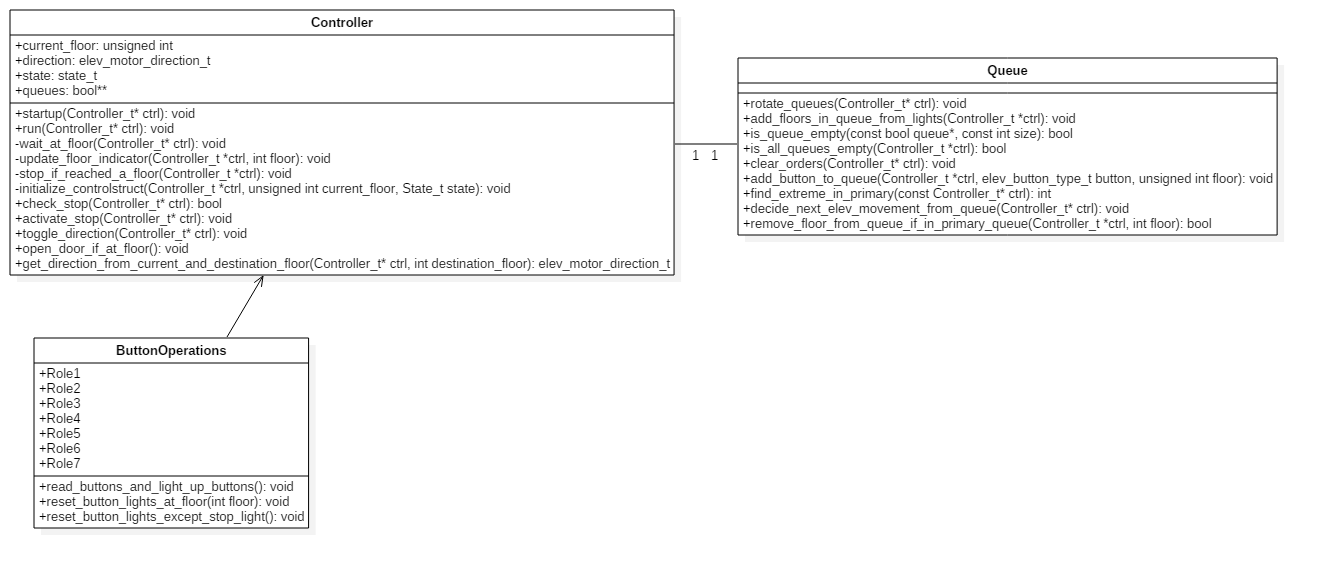
\includegraphics[width=\textwidth]{./Model__Main_0.png}


\section{Sequence Diagram}
\begin{enumerate}
\item Heisen står tom og stille i 2. etasje med døra åpen
\item En person signaliserer fra 1. etasje at hun ønsker transport oppover
\item Når heisen kommer, bestiller hun transport til 3. etasje
\item Scenariet avsluttes når heisen befinner seg i 3. etasje og heisdøra åpnes
\end{enumerate}
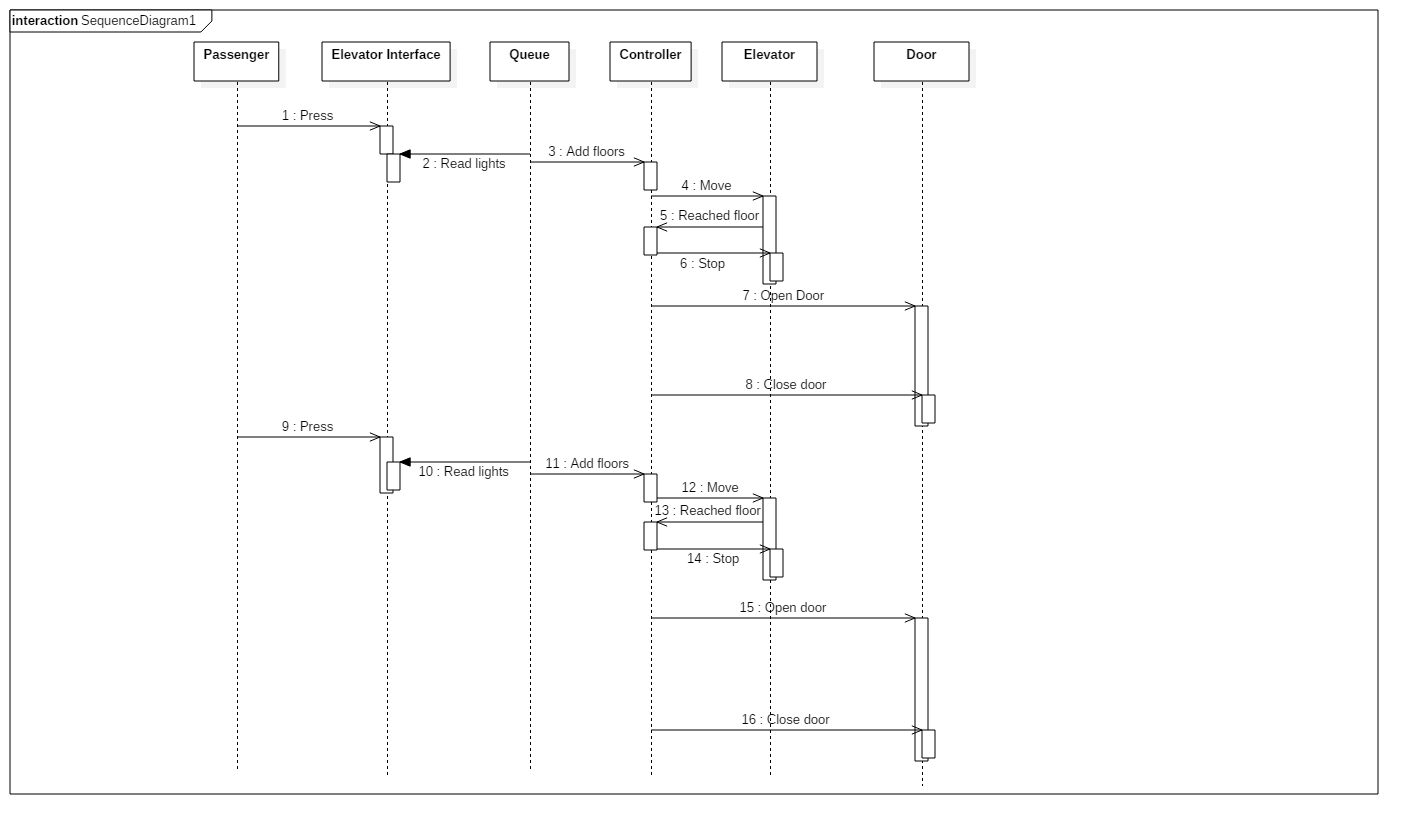
\includegraphics[width=\textwidth]{./Model__ButtonOperations__Interaction1__SequenceDiagram1_6.png}

\section{Use Case Diagram}

Main success scenario with extensions
\begin{enumerate}
	\item Customer presses up/down-button.
	\item System orders elevator to go to customer floor and opens door.
	\begin{enumerate}
	\item Elevator is going the opposite direction
		\begin{enumerate}
	\item Elevator doesn't stop unless someone wants to go down, or someone in the elevator has selected the floor.
	\item When Elevator is going the same direction as desired floor movement ->  2.
			\end{enumerate}
						\end{enumerate}
	\item Customer goes in the elevator
	\item Customer presses a floor button to select a floor.
	\begin{enumerate}
	\item Stop-button is pressed
		\begin{enumerate}
	\item Reset all buttons
	\item  If on floor -> open door
	\item   -> 4.c.ii
			\end{enumerate}
	\item  Presses multiple buttons
		\begin{enumerate}
	\item  Add selected floors in queue.
			\end{enumerate}
	\item  Presses the same floor button as current floor.
		\begin{enumerate}
	\item  "Close door"-timer resets
			\end{enumerate}
	\item  Doesn't press button.
		\begin{enumerate}
	\item  Close door after three seconds.
	\item  Wait until button press. If
			\begin{enumerate}
	\item  Up/down -> 1.
	\item  Floor button -> 3.
				\end{enumerate}
									\end{enumerate}
				\end{enumerate}
	\item  System closes door after three seconds
	\item  Moves in desired direction.
	\begin{enumerate}
	\item  Presses one or more buttons
		\begin{enumerate}
	\item Stop-button is pressed -> 4.a.i
	\item  Multiple buttons ->  Add selected floors in queue.
			\end{enumerate}
			\end{enumerate}
	\item Elevator stops in next selected floor on the way
	\begin{enumerate}
	\item  Presses one or more buttons
		\begin{enumerate}
	\item  Stop-button is pressed -> 4.a.i
	\item  Multiple buttons ->  Add selected floors in queue.
		\end{enumerate}
	\end{enumerate}
	\item  System opens door.
	\begin{enumerate}
	\item  Presses one or more buttons
		\begin{enumerate}
	\item  Stop-button is pressed -> 4.a.i
	\item  Same floor as current ->  4.c.i
	\item  Multiple buttons-> 4.b.i
			\end{enumerate}
	\item   If
		\begin{enumerate}
	\item  queue empty ->  4.d.i
	\item  Else -> 5.
		\end{enumerate}
		\end{enumerate}
\end{enumerate}
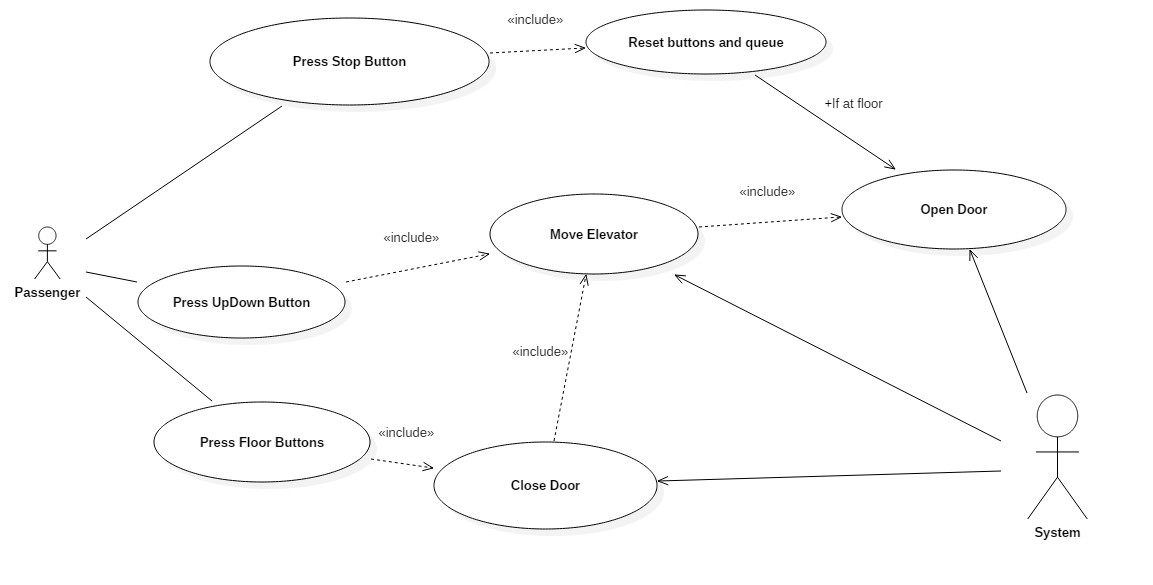
\includegraphics[width=\textwidth]{./Model1__UseCase_1.png}

\section{State Diagram}
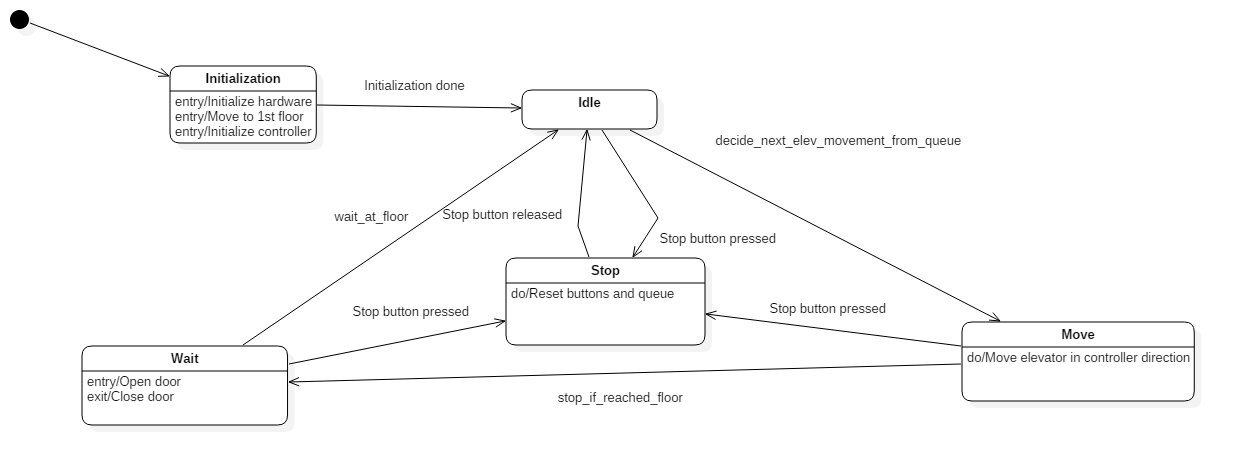
\includegraphics[width=\textwidth]{./StateMachine1__StatechartDiagram1_3.png}

\section{Activity Diagram}
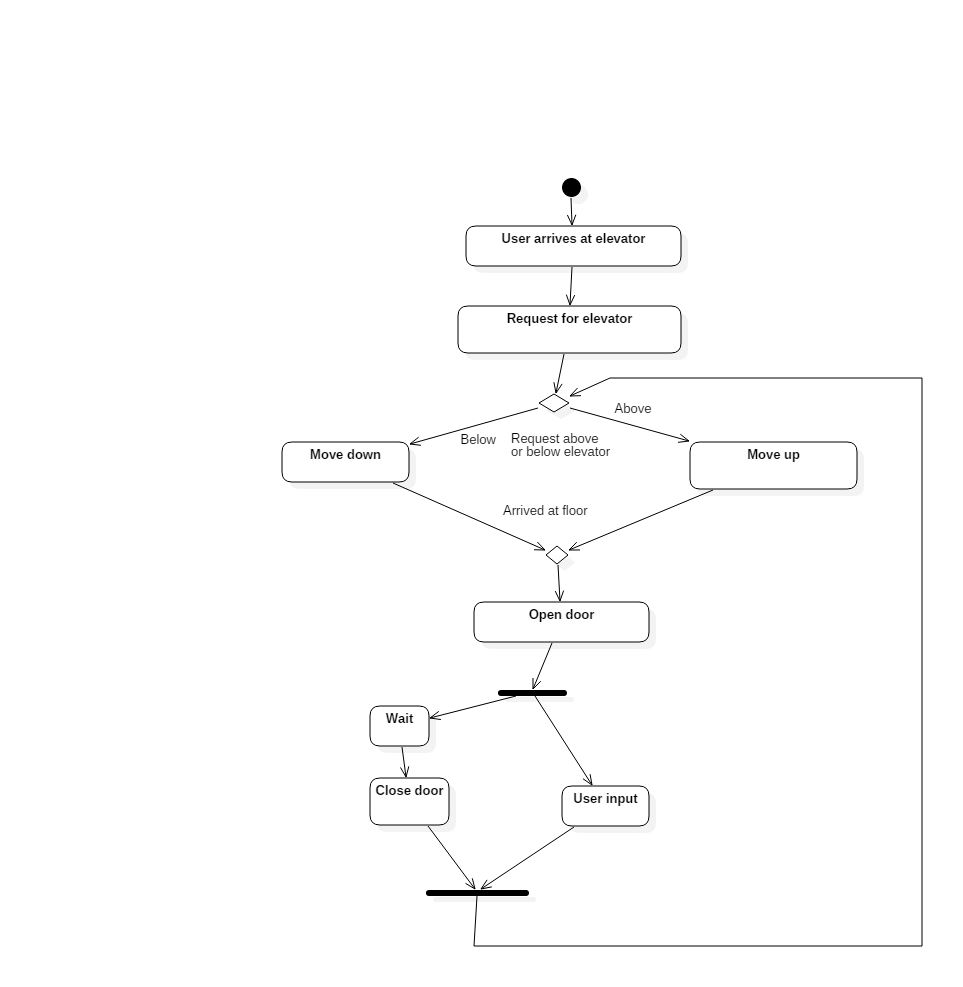
\includegraphics[width=\textwidth]{./Activity1__ActivityDiagram1_4.png}

\section{Communication Diagram}
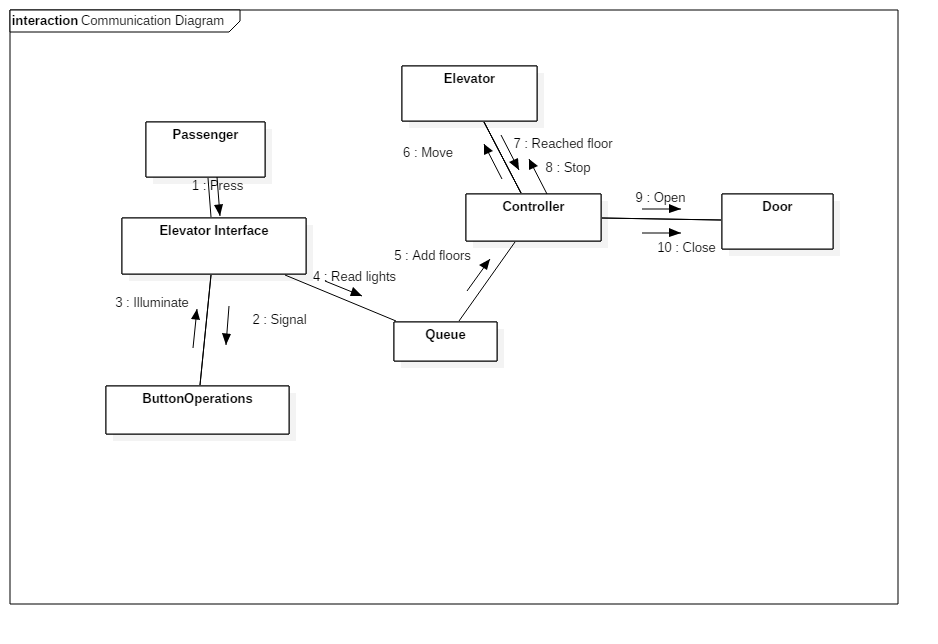
\includegraphics[width=\textwidth]{./Collaboration2__Interaction1__Communication_Diagram_5.png}

\section{Timing Diagram}
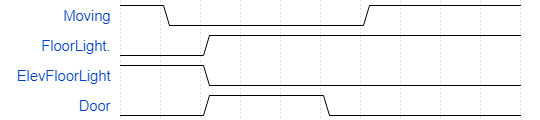
\includegraphics[width=\textwidth]{./Timing_Diagram.png}
\end{document}
